%%%%%%%%%%%%%%%%%%%%%%%%%%%%%%%%%%%%%%%%%%%%%%%%%%%%%%%%%%%%
%%  This Beamer template was created by Cameron Bracken.
%%  Anyone can freely use or modify it for any purpose
%%  without attribution.
%%
%%  Last Modified: January 9, 2009
%%

\documentclass[xcolor=x11names,compress]{beamer}

%% General document %%%%%%%%%%%%%%%%%%%%%%%%%%%%%%%%%%
\usepackage{graphicx}
\usepackage{tikz}
\usepackage[french]{babel}
\usepackage[T1]{fontenc}
\usepackage[utf8]{inputenc}
\usepackage{array}
\usetikzlibrary{decorations.fractals}
%%%%%%%%%%%%%%%%%%%%%%%%%%%%%%%%%%%%%%%%%%%%%%%%%%%%%%


%% Beamer Layout %%%%%%%%%%%%%%%%%%%%%%%%%%%%%%%%%%
\useoutertheme[subsection=false,shadow]{miniframes}
\useinnertheme{default}
\usefonttheme{serif}
\usepackage{palatino}

\setbeamerfont{title like}{shape=\scshape}
\setbeamerfont{frametitle}{shape=\scshape}

\setbeamercolor*{lower separation line head}{bg=DeepSkyBlue4} 
\setbeamercolor*{normal text}{fg=black,bg=white} 
\setbeamercolor*{alerted text}{fg=red} 
\setbeamercolor*{example text}{fg=black} 
\setbeamercolor*{structure}{fg=black} 
 
\setbeamercolor*{palette tertiary}{fg=black,bg=black!10} 
\setbeamercolor*{palette quaternary}{fg=black,bg=black!10} 

\setbeamertemplate{footline}
{%
  \leavevmode%
  \hbox{\begin{beamercolorbox}[wd=.16\paperwidth,ht=2.5ex,dp=1.125ex,leftskip=.3cm%
	plus1fill,rightskip=.3cm,center]{author in head/foot}%
    \usebeamerfont{author in head/foot}Mathieu Soum
  \end{beamercolorbox}%
  \begin{beamercolorbox}[wd=.77\paperwidth,ht=2.5ex,dp=1.125ex,leftskip=.3cm,rightskip=.3cm%
	plus1fil,center]{author in head/foot}%
	\usebeamerfont{title in head/foot}Elaastic -- Conception et diffusion de
	contenu pédagogique
  \end{beamercolorbox}%
  \begin{beamercolorbox}[wd=.07\paperwidth,ht=2.5ex,dp=1.125ex,leftskip=.3cm,rightskip=.3cm%
	plus1fil,center]{author in head/foot}%
	\usebeamerfont{frame number in head/foot}\insertframenumber
  \end{beamercolorbox}}%
  \vskip0pt%
}

\renewcommand{\(}{\begin{columns}}
\renewcommand{\)}{\end{columns}}
\newcommand{\<}[1]{\begin{column}{#1}}
\renewcommand{\>}{\end{column}}
%%%%%%%%%%%%%%%%%%%%%%%%%%%%%%%%%%%%%%%%%%%%%%%%%%

\setbeamercovered{invisible}

\AtBeginSection[]{%
  \begin{frame}<beamer>
	\tableofcontents[currentsection]
  \end{frame}
}


\begin{document}


%%%%%%%%%%%%%%%%%%%%%%%%%%%%%%%%%%%%%%%%%%%%%%%%%%%%%%
%%%%%%%%%%%%%%%%%%%%%%%%%%%%%%%%%%%%%%%%%%%%%%%%%%%%%%
\begin{frame}
\title{Application Java EE dédiée à la conception et à la diffusion de supports
pédagogiques}
%\subtitle{SUBTITLE}
\author{
	Mathieu Soum\\
	{\it Université Paul Sabatier}\\
	{\it Master 1 -- Développement Logiciel}\\
    \vspace{5px}
	Stage réalisé chez TiceTime
  \vspace{-15px}
}
\date{
	{
	  \includegraphics[scale=0.13]{images/ticetime}\hspace{75px}\includegraphics[scale=0.37]{images/ups}
	}
	\\
	\vspace{15px}
	Année universitaire 2013 - 2014
}
\titlepage
\end{frame}

%%%%%%%%%%%%%%%%%%%%%%%%%%%%%%%%%%%%%%%%%%%%%%%%%%%%%%
%%%%%%%%%%%%%%%%%%%%%%%%%%%%%%%%%%%%%%%%%%%%%%%%%%%%%%
\begin{frame}
\tableofcontents
\end{frame}

%%%%%%%%%%%%%%%%%%%%%%%%%%%%%%%%%%%%%%%%%%%%%%%%%%%%%%
%%%%%%%%%%%%%%%%%%%%%%%%%%%%%%%%%%%%%%%%%%%%%%%%%%%%%%
\section{\scshape Contexte}
\begin{frame}{Vue d'ensemble}
  \begin{center}
	\onslide<1->{\includegraphics[scale=0.15]{images/ticetime}}
	\pause
	\vfill
	\onslide<2->{
\includegraphics[scale=0.19]{images/elaastic_logo}}
	\vfill
	\onslide<3->{
	  \hfill
	  \includegraphics[scale=0.6]{images/grails}
	  \hfill
	  \includegraphics[scale=0.1]{images/angularjs}
	  \hfill\hfill
	}
  \end{center}
\end{frame}

\begin{frame}
  \begin{center}
	\includegraphics[scale=0.23]{images/screenshot_elaastic}
  \end{center}
\end{frame}

\begin{frame}{Un peu d'agilité}
  \begin{itemize}
	\item Daily meeting
	\item Story $\rightarrow$ Tâches $\rightarrow$ Sous-tâche
	\item Tableau Kanban
  \end{itemize}
\end{frame}

%%%%%%%%%%%%%%%%%%%%%%%%%%%%%%%%%%%%%%%%%%%%%%%%%%%%%%
%%%%%%%%%%%%%%%%%%%%%%%%%%%%%%%%%%%%%%%%%%%%%%%%%%%%%%
\section{\scshape Outils et méthodologie}
\begin{frame}{Les outils}
  \begin{center}
	\includegraphics[scale=0.45]{images/tools}
  \end{center}
\end{frame}

\begin{frame}{La méthodologie 1/3}{Jira}
  \begin{center}
	\includegraphics[scale=0.25]{images/jira}\\
	Story $\rightarrow$ Tâches $\rightarrow$ Sous-tâches\\
	\vfill
	\includegraphics[scale=0.3]{images/jira_kanban}
  \end{center}
\end{frame}

\begin{frame}{La méthodologie 2/3}{Git}
  \begin{center}
	Branches git\\
	{\small \tt quadruplet/nom fiche/ID fiche/modifieur/numéro}\\
	\vfill
  \end{center}
  \pause
  \begin{flushleft}
	{\small \tt msou/Unit\_as\_interactive\_question/EL-288/1}\\
	{\small \tt msou/Unit\_as\_interactive\_question/EL-288/review/2}\\
	{\small \tt msou/Unit\_as\_interactive\_question/EL-288/ready/3}
  \end{flushleft}
\end{frame}

\begin{frame}{La méthodologie 3/3}{Les tests}
  \begin{center}
	\begin{itemize}
	  \item Couverture maximale
	  \item Spock
	  \begin{itemize}
		  \item Test = Spécification
		  \item given, when, then
		  \item Mock objects (simulation de comportement)
	  \end{itemize}
	\end{itemize}
  \end{center}
\end{frame}


%%%%%%%%%%%%%%%%%%%%%%%%%%%%%%%%%%%%%%%%%%%%%%%%%%%%%%
%%%%%%%%%%%%%%%%%%%%%%%%%%%%%%%%%%%%%%%%%%%%%%%%%%%%%%
\section{\scshape Fonctionnalités}
\begin{frame}{IMS Content Packaging}{}
  {\em En tant qu'}utilisateur final d'Elaastic ;\\
  {\em Je veux} exporter mon cours dans le format IMS Content Packaging ;\\
  {\em Afin de} pouvoir l'importer dans le LMS de mon établissement.
\end{frame}

\begin{frame}{IMS Content Packaging}{Définition}
  \only<1,3>{\begin{itemize}
	\item Format standard
	\item IMS Global Learning Consortium
	\item Compatible Moodle
  \end{itemize} }
  \only<2>{ \includegraphics[scale=0.23]{images/ims_moodle} }
  \pause
  \only<1,3>{\begin{itemize}
	\item Archive zip
	\item Manifest XML
	\item Resources
  \end{itemize} }
\end{frame}

\begin{frame}{IMS Content Packaging}{L'archive zip}
  \begin{itemize}
	\item imsmanifest.xml
	\item content
	  \begin{itemize}
		\item unit1.1.html
		\item unit1.2.html
		\item unit2.1.html
		\item \ldots
	  \end{itemize}
	\item resource
	  \begin{itemize}
		\item picture1.jpg
		\item picture2.jpg
		\item \ldots
	  \end{itemize}
  \end{itemize}
\end{frame}

\begin{frame}{IMS Content Packaging}{Le manifest}
  \begin{enumerate}
	\item Meta-données
	  \pause
	\item Structure
	  \pause
	\item Ressources
	  \pause
	\item Validation
  \end{enumerate}
\end{frame}

\begin{frame}{WebDAV}
  \begin{itemize}
	\item {\bf Web D}istributed {\bf A}uthoring and {\bf V}ersioning
	\item Extension HTTP
	\item Opérations sur des fichiers
  \end{itemize}
  \pause
  \vfill
  \begin{center}
	\includegraphics[scale=0.5]{images/moodle}
  \end{center}
  \vfill
\end{frame}

\begin{frame}{Artéfact}{Le problème}
  \begin{itemize}
	\item Export dans plusieurs formats
	\item Temps d'export trop important !
  \end{itemize}
  \vfill
  \begin{center}
	Système de cache $\Rightarrow$ Réponse plus rapide
  \end{center}
  \vfill
\end{frame}

\begin{frame}{Artéfact}{Solition mise en place}
  Artéfact
  \begin{itemize}
	\item Cours
	\item Version du cours
	\item Format
  \end{itemize}
  \vfill
  \begin{center}
	Binaire stocké en base $\Rightarrow$ Pas besoin de transformation
  \end{center}
  \vfill
\end{frame}

\begin{frame}{Diffusion}{Le concept}
  \begin{center}
	Accès externe à une version de cours dans un format exporté
	\vfill
	\includegraphics[scale=0.22]{images/diffusion}
  \end{center}
\end{frame}

\begin{frame}{Diffusion}{Fonctionnement}
  \begin{center}
	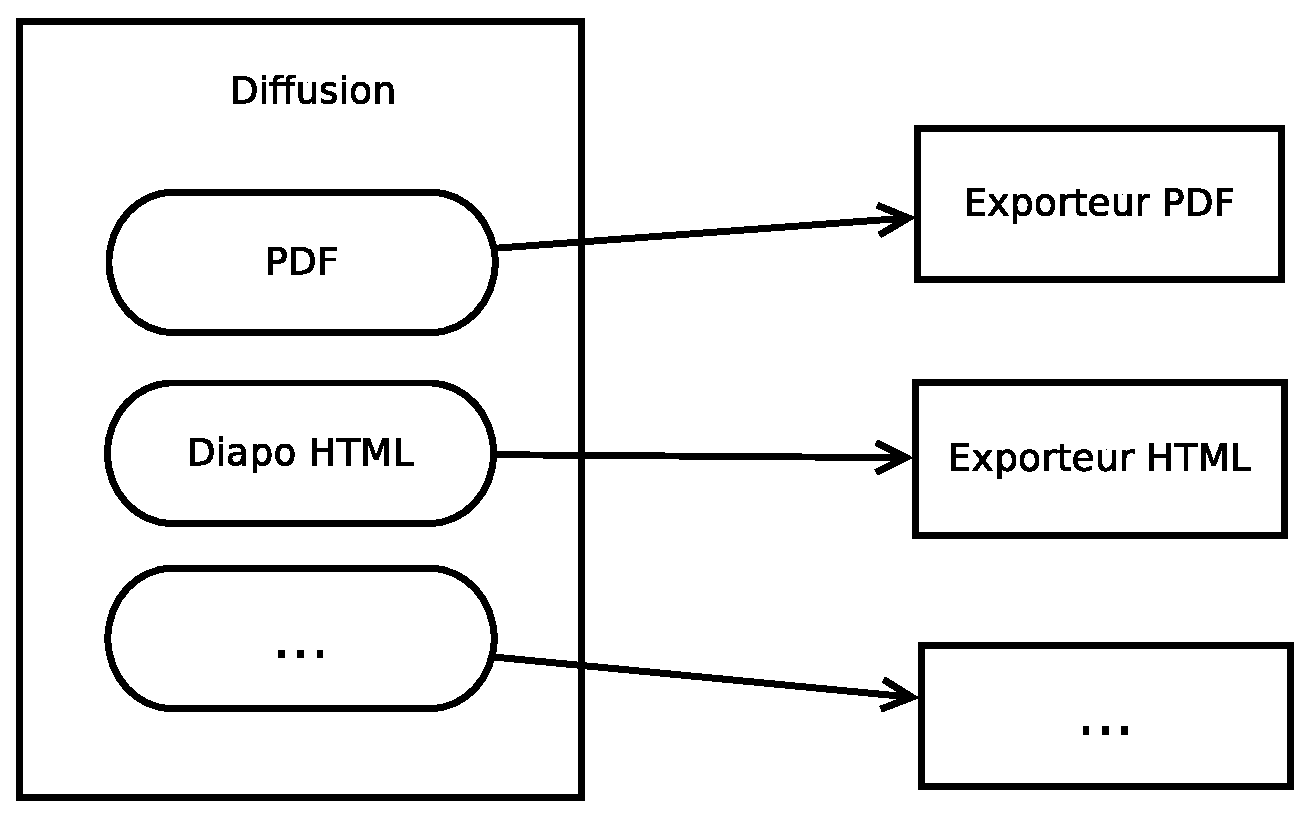
\includegraphics[scale=0.25]{images/diffusion_schema}
	\vfill
	\pause
	Groupes $\rightarrow$ Même cours $\rightarrow$ Artéfact
  \end{center}
\end{frame}

\begin{frame}{Questions intéractives}{Tsaap-notes}
  \begin{center}
	\includegraphics[scale=0.4]{images/tsaap}
	\vfill
	\begin{itemize}
	  \item Prise de notes collaboratives
	  \item Questions intéractives
	  \item Feedback temps réel
	\end{itemize}
	\vfill
	Langage Moodle GIFT
  \end{center}
\end{frame}

\begin{frame}{Questions intéractives}{Elaastic}
  \begin{itemize}
	\item Intégration Tsaap-notes (plugin)
	\item \og Unité question \fg{}
	\item Rendu dynamique/statique
  \end{itemize}
  \pause
  \vfill
  \begin{itemize}
	\item Docbook {\tt @role=question}
	\item Dynamique $\rightarrow$ {\tt <form>} + API REST
	\item Statique $\rightarrow$ Liste
  \end{itemize}
\end{frame}


%%%%%%%%%%%%%%%%%%%%%%%%%%%%%%%%%%%%%%%%%%%%%%%%%%%%%%
%%%%%%%%%%%%%%%%%%%%%%%%%%%%%%%%%%%%%%%%%%%%%%%%%%%%%%
\section{\scshape Bilan}
\begin{frame}{Expérience professionnelle}
  \vfill
  \begin{itemize}
	\item Projet Web
	\item Framework Grails
	\item Spécification par les tests
	\item Pratiques agiles
  \end{itemize}
  \vfill
\end{frame}

\begin{frame}{Apports personnels}
  \vfill
  \begin{itemize}
	\item Expérience Web
	\item Formation complémentaire
  \end{itemize}
  \vfill
  \begin{itemize}
	\item Client léger vs client lourd
	\item Langage natif
  \end{itemize}
\end{frame}

%%%%%%%%%%%%%%%%%%%%%%%%%%%%%%%%%%%%%%%%%%%%%%%%%%%%%%
%%%%%%%%%%%%%%%%%%%%%%%%%%%%%%%%%%%%%%%%%%%%%%%%%%%%%%
\section*{}

\begin{frame}
  \title{Application Java EE dédiée à la conception et à la diffusion de supports
  pédagogiques}
  %\subtitle{SUBTITLE}
  \author{
	  Mathieu Soum\\
	  {\it Université Paul Sabatier}\\
	  {\it Master 1 -- Développement Logiciel}\\
	  \vspace{5px}
	  Stage réalisé chez TiceTime
	\vspace{-15px}
  }
  \date{
	  {
		\includegraphics[scale=0.13]{images/ticetime}\hspace{75px}\includegraphics[scale=0.37]{images/ups}
	  }
	  \\
	  \vspace{15px}
	  Année universitaire 2013 - 2014
  }
  \titlepage
\end{frame}

\begin{frame}{Mock objects}
  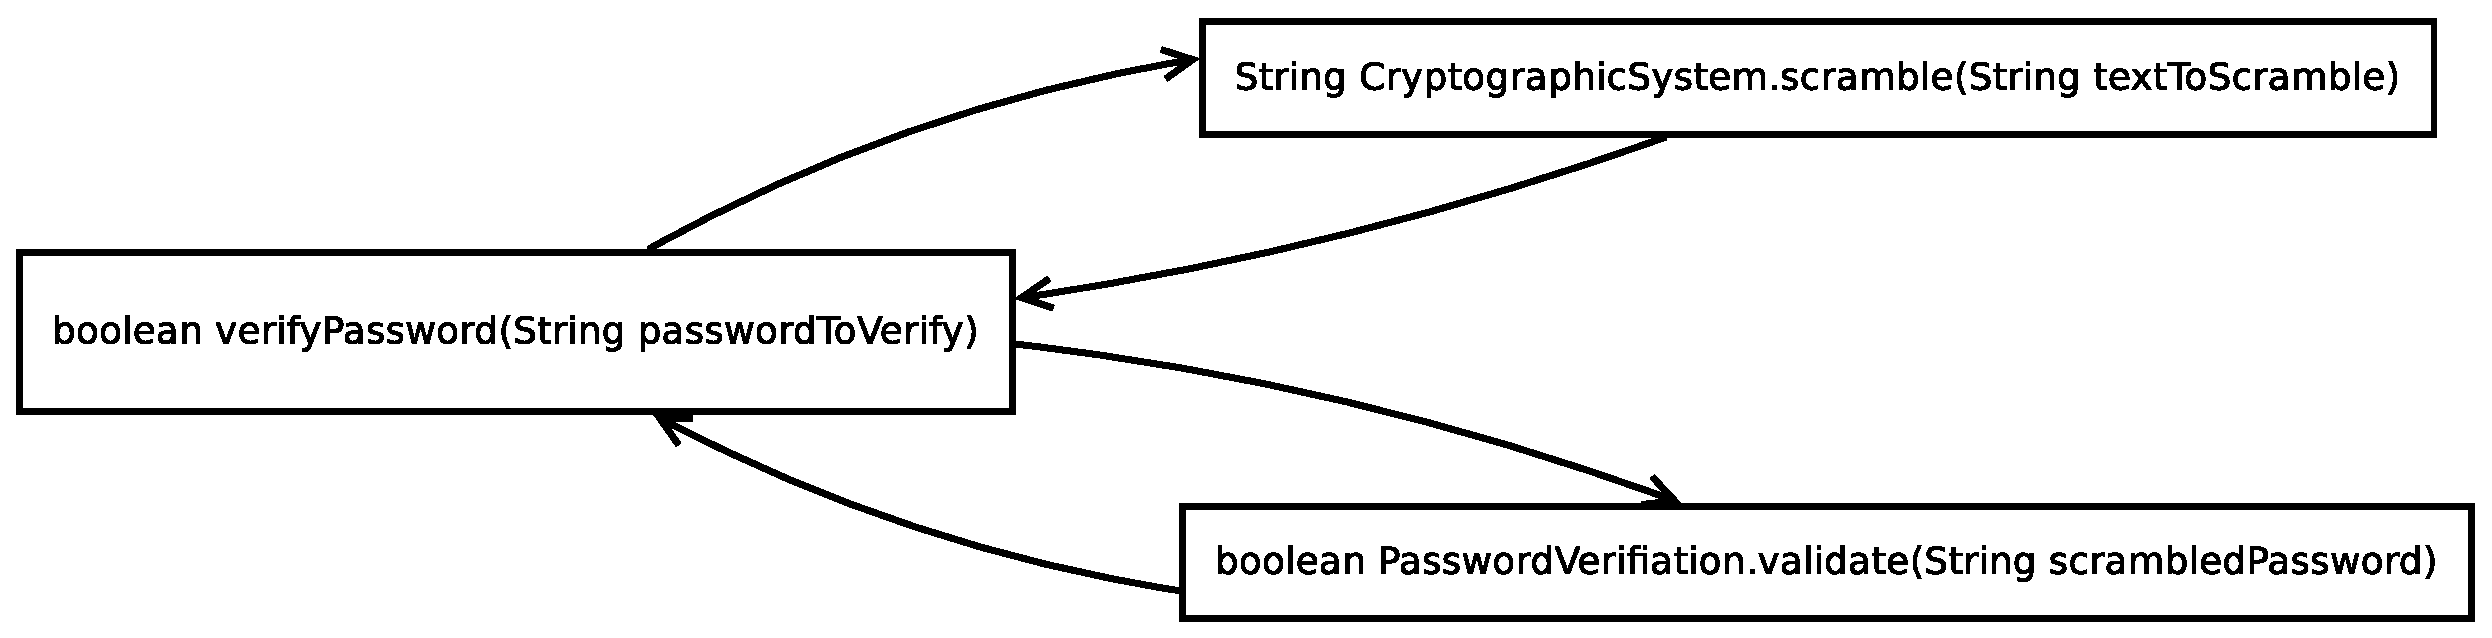
\includegraphics[scale=0.25]{images/mockObj}
\end{frame}

\begin{frame}{Structure d'application}
  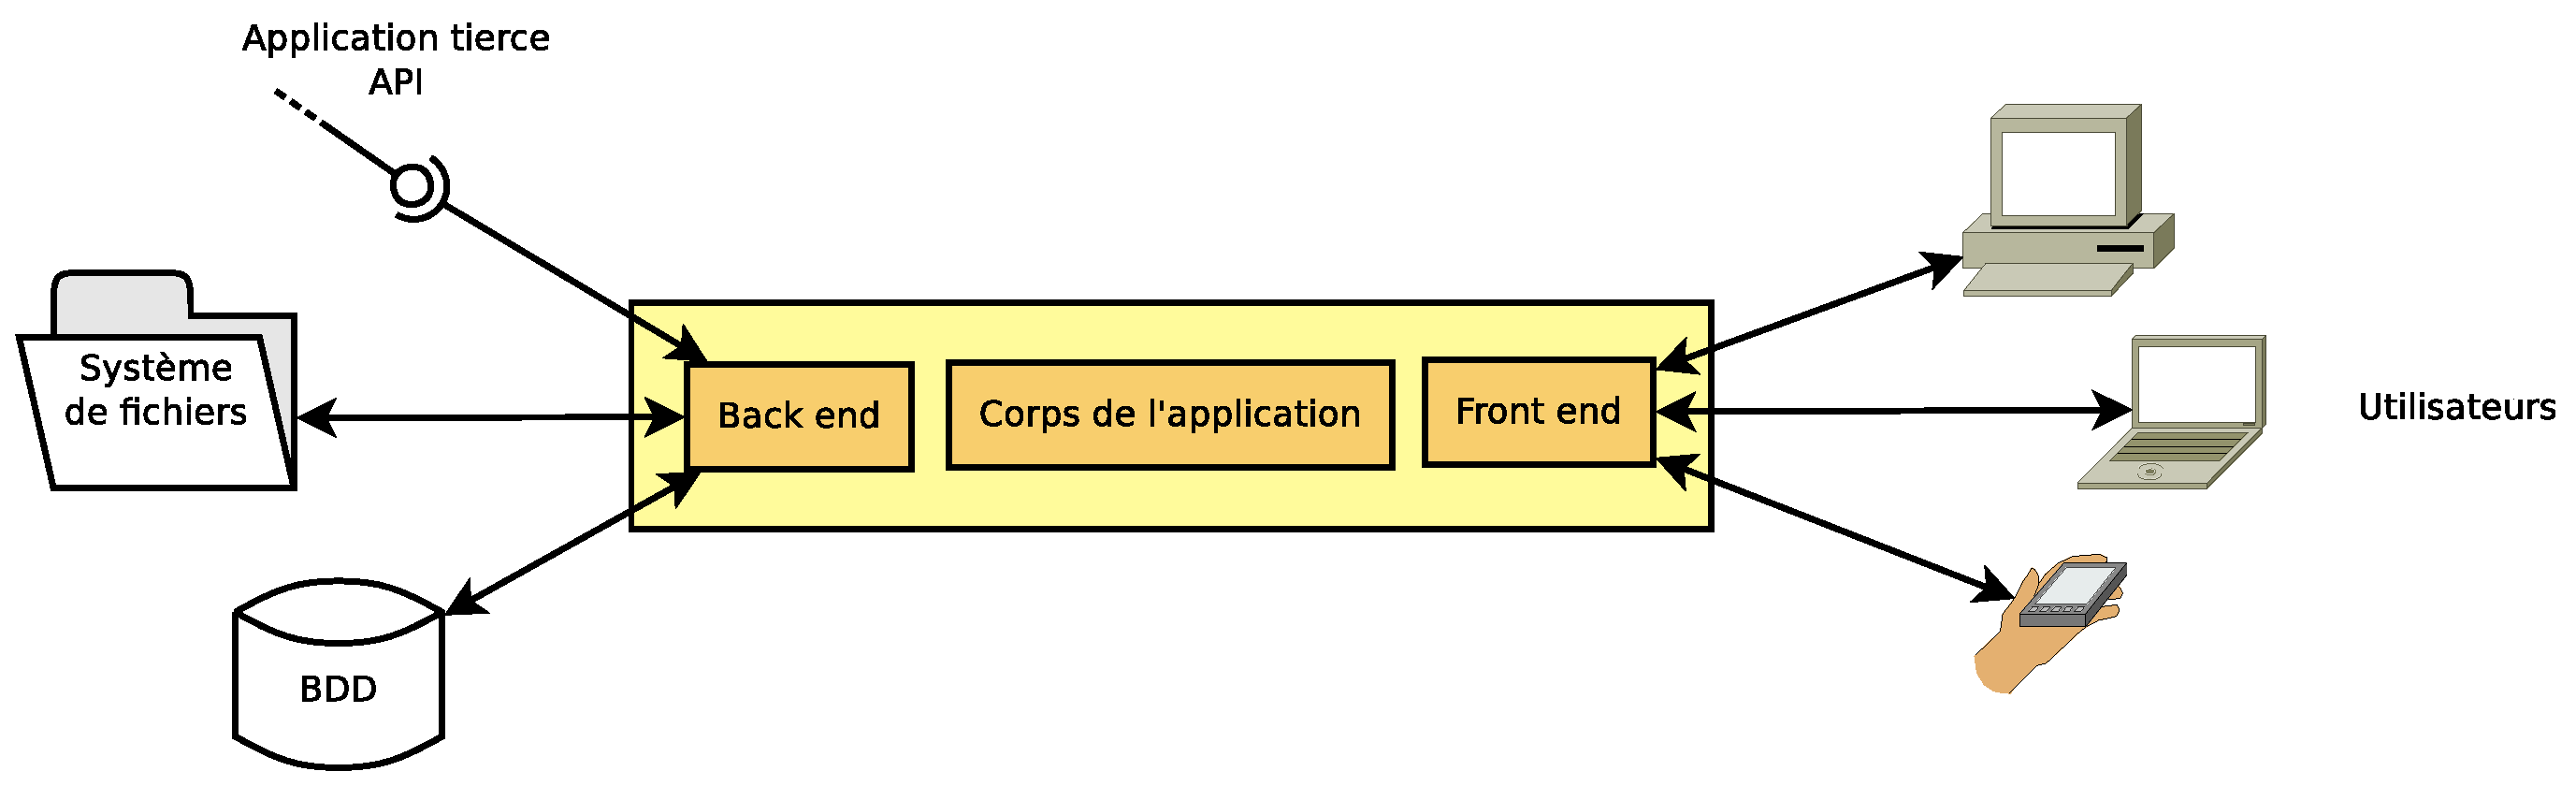
\includegraphics[scale=0.24]{images/webapp}
\end{frame}

\end{document}
